%!TEX root = ../thesis.tex
\chapter{Medical Fundamentals}
\label{chap:medFund}


\section{Atrial Anatomy and Physiology}
\label{sec:anatomyPhysiology}

We try to support the diagnosis of arrhythmias like \ac{AFib}. \Ac{AFlut} already is very well understood.


\subsection{Electrophysiology}
\label{sec:anatomyPhysiology:elphy}

The course of an \ac{AP} is important to know.

\begin{figure}[tb]
 \centering
 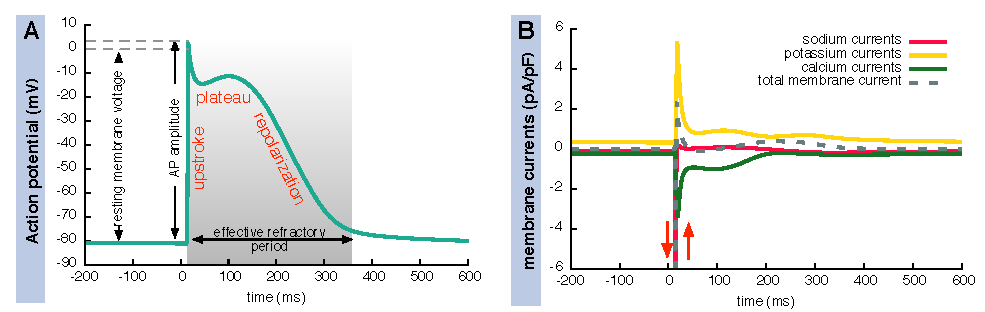
\includegraphics[width=\textwidth]{Funda-Med-AP}
 \caption{The course of the transmembrane voltage V$_\textnormal{m}$ during a cardiac \ac{AP} with its different phases (A) and the membrane currents carried by the different ions (B). The sodium current reaches an amplitude of $\approx$--70\,pA/pF. The calcium exchange with the sarcoplasmic reticulum is not considered. Courses were computed using the Courtemanche \etal model~\cite{courtemanche98}. Figure inspired by~\cite{schmidt10a}.}
 \label{fig:med:AP}
\end{figure}

\begin{figure}[ht]
\centering
\subfloat[Vector label (PDF format).]
	{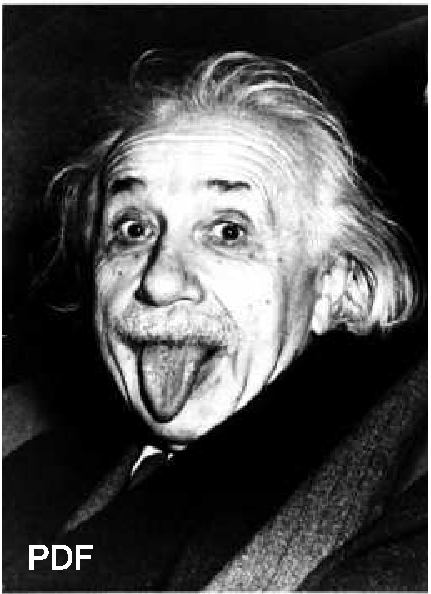
\includegraphics[width=0.4\textwidth]{einsteinlabelVEC}}
\hspace{0.05\textwidth}
\subfloat[Pixel label (PNG format).]
	{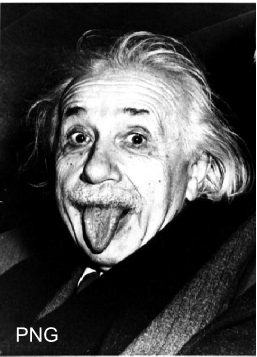
\includegraphics[width=0.4\textwidth]{einsteinlabelPIX}}
\caption{Photographs of different formats. One is vector~(a), one is pixel-base~(b).}
 \label{fig:med:einsteinComparsion}
\end{figure}

\Fig{fig:med:AP} is an example of a vector graphics figure. You can zoom in as you want, the figure will always stay sharp. This is the preferable format for all line drawings (\eg plots). Photographs are always saved as pixel graphics. However, labels can be added in a vector format (compare Figure~\ref{fig:med:einsteinComparsion}).\\
If you want to include a list of figures and a list of tables in your work, you probably want to provide short captions in square brackets as well. The
